\chapter{Database}

\section{Analysis}

In the beginning of the project, it was determined that the given data files always should be parsed in real time, when needed on the frontend. During the analysis of how to handle the different data, however, it was quickly found that this solution would be clumsy to implement, inflexible and generally inefficient.\\
For proper data management a database was to be used. Because of the large quantity of the data per file (e.g. a csv single file contains over 72.000 rows), the size of the database can and will increase very rapidly if the application is used on regular basis, and this should be taken into consideration when designing it.\\\\
For safety reasons, the application should also contain user authentication in order to get certain administration privileges (such as file CUD). The database should therefore also handle data management for users.\\

\section{Design}
All tables will contain an \textsf{id} column, such that all rows in the same table are unique. This also makes it easy to fetch and perform actions for a specific row.\\\\
\textsf{users} table should at minimum contain the columns \textsf{username, password} and \textsf{email}.\\
\textsf{files} table should at minimum contain the columns \textsf{name, latitude, longitude, path, type} and \textsf{offset}.\\ Also, as it would be convenient to know who uploaded the file, a \textsf{user\_id} field should also be created.\\
There will be a table for all supported file types (currently \textsf{csv} and \textsf{wrk}). \textsf{csv} table should contain columns as stated in SEKTION 3.3.4, and \textsf{wrk} as defined by the VRIS file format. Besides these columns, all file type tables should contain a \textsf{file\_id} field so all data is related to the source file (in the database).\\\\
As the database should be able to handle a large amount of data, it is crucial that all columns are of correct and optimal data types, e.g. \textsf{id} columns are either \textit{int} or \textsf{bigint} and are \textsf{unsigned}. By comparison, \textsf{unsigned int} can take the maximum value $2^{32}-1 (\textasciitilde 4.29 \cdot 10^{9})$ while it for \textsf{unsigned bigint} is $ 2^{64}-1 (\textasciitilde 18.45 \cdot 10^{18})$.

\section{Implementation}

Below is a diagram of the database has been implemented based on the analysis and design:\\
\begin{figure}[htbp]
   \centering
   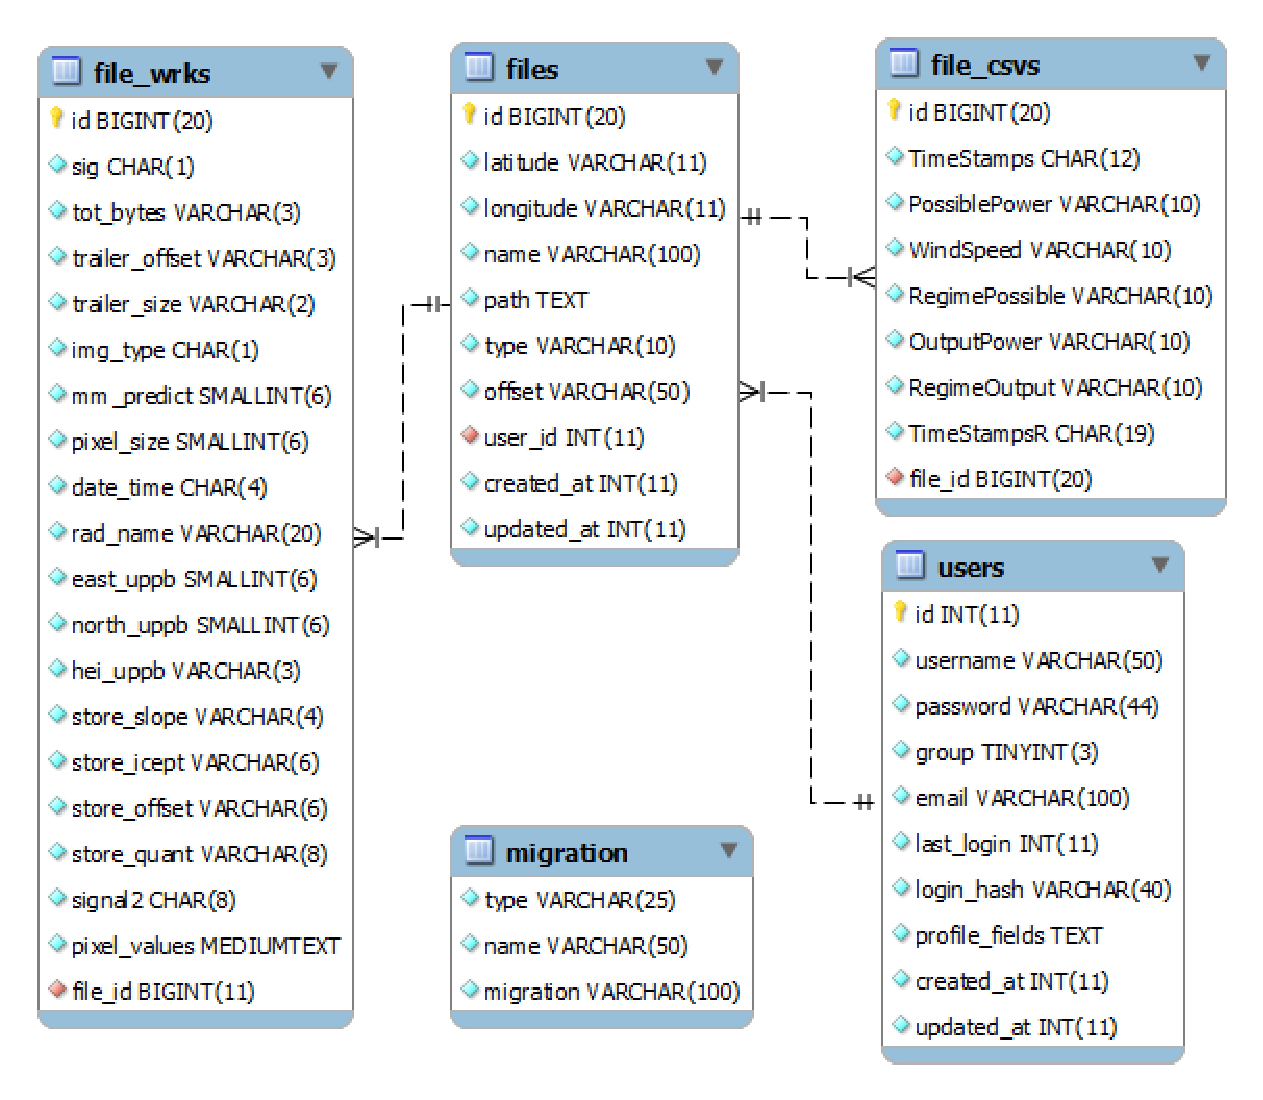
\includegraphics[width=1\linewidth]{figure/db}
   \caption{Database Diagram}
\end{figure}
FuelPHP contains a \textsf{migration} tool that lets one create revisions for the database, hence easy deployment of changes. This tool has been used to create all tables, and therefore the \textsf{migration} table is used to keep track of revisions.\\\\

All tables use \textsf{InnoDB}, because this engine make it possible to create sql relations. This means that if a table has a foreign key (i.e. a key that identifies a row in another table), one can create actions for what should happen to the rows in the current table, if the related row in the other table is \textsf{updated} or \textsf{deleted}.\\
These relations can be seen in the diagram. The relations and actions is stated by sql as:\\\\

\begin{lstlisting}[language=sql]
ALTER TABLE `files`
  ADD CONSTRAINT `files\_ibfk\_1` FOREIGN KEY (`user_id`) REFERENCES `users` (`id`) ON DELETE NO ACTION ON UPDATE NO ACTION;

ALTER TABLE `file\_csvs`
  ADD CONSTRAINT `file\_csvs\_ibfk\_1` FOREIGN KEY (`file_id`) REFERENCES `files` (`id`) ON DELETE CASCADE ON UPDATE NO ACTION;

ALTER TABLE `file\_wrks`
  ADD CONSTRAINT `file\_wrks\_ibfk\_1` FOREIGN KEY (`file_id`) REFERENCES `files` (`id`) ON DELETE CASCADE ON UPDATE NO ACTION;
\end{lstlisting}

\section{Optimisation}

In FuelPHP it is possible to create model relations that are similar to sql relations with actions, but easier to manage and at the same time less efficient (though generally adequate). This method was used initially, but performance was found to be too bad, e.g. it would take too much time to cascade delete all the csv rows related to the file selected for deletion, eventually leading to a time out by the server. The time out limit can be changed by the server manager, but it was easier and - as stated before - more efficient to make relation actions in sql. Relations are still present at model level, but actions have been turned off.
